% generated by make_combined.py from stage7_robustness_external/stage7.tex; do not edit
\section{Stage 7 --- How robust is the location law?}\label{sec:stage7}

\stagebox{\textbf{In one sentence.} The location law does not depend on how masking is implemented --- black fill, a
blurred background, cropping to the lesion box and cropping the masked image all give a positive crossover in all four
real-artifact cohorts (\sSevenNPrimOK{} of \sSevenNPrim{}, Holm) --- it is graded rather than a threshold effect (the mask
gain falls monotonically with the real overlap $r$ in all four cohorts, and for hair turns into harm above $r\approx$
\sSevenZeroIsic), it reappears on an external, patient-level test set at natural prevalence (ISIC 2019 $\to$ ISIC 2020:
masking raises overall AUROC but lowers it on the shortcut-conflicting pairs), and the two-parameter theory of Stage~5,
tested prospectively on \sSevenTN{} cells that did not exist when the test was registered, met its registered criterion for
quantitative prediction.}
\subsection{Where this stage starts}
Stages~1--6 established the location law --- ROI masking removes an out-of-ROI shortcut and keeps, or amplifies, an
in-ROI one --- in controlled sweeps (Stage~2), with real artifacts in four cohorts (Stage~3), against the alternative that
different images carry the artifact in the two traps (Stage~4), on natural test sets and across encoders, with a theory
that closely matches held-out results (Stage~5), and they built remedies around it (Stage~6). Four objections remained
open, each of which a reviewer can raise against the central claim:
\begin{enumerate}[leftmargin=*]\itemsep1pt
\item \emph{``Mean-colour fill is one implementation.''} Clinical pipelines crop to the lesion or use black
backgrounds; the law might be a property of the particular fill used in Stages~1--6.
\item \emph{``Trap~A ($r\ge0.5$) and Trap~B ($r<0.1$) are two hand-picked extremes.''} The crossover might be a
dichotomy produced by the thresholds rather than a graded dependence on where the artifact lies.
\item \emph{``Resampled traps are artificial and the data are internal.''} The natural test sets of Stage~5 were
held-out parts of the training datasets; the ISIC 2020 validation of Stage~5 still used resampled traps.
\item \emph{``The theory was checked only on results that already existed.''} Stage~5's test of the theory was
retrospective.
\end{enumerate}
This stage answers each with one pre-registered analysis (R8--R11).

\subsection{Questions}
\begin{enumerate}[label=\textbf{Q7\alph*},leftmargin=*]\itemsep1pt
\item Does the crossover hold for other masking implementations, and do implementations that remove out-of-ROI
content only partly give a weaker location effect?
\item Does the mask gain fall continuously as more of a real artifact lies inside the ROI?
\item Trained on one dataset and tested on another collected from other patients, at natural prevalence and without
resampling, does masking harm the cases that conflict with the in-lesion hair association?
\item Does the theory predict results it has never seen, by the rule registered before they existed?
\end{enumerate}
\paragraph{Design decisions} \emph{One registration for the whole stage} (Table~\ref{s7:tab:exp}), committed before any
feature, cell count or model of this stage existed; every hypothesis is reported whichever way it went.
\emph{Identical environments}: every trap of R8 and R9 uses the cohorts, artifact definitions, matching, seeds, folds,
heads and thresholds of Stage~3, so the new arms are paired with ERM on the same images. \emph{A reproducibility gate}: each
R8 run re-fits ERM and mean-colour masking and had to reproduce the stored Stage~3 runs within 0.03 AUROC before any new
result was read; the largest difference was \sSevenReproMax. \emph{Counts before models}: the dose-response bins, their
count gate and the merge rule were applied and committed (\sSevenCommitCounts) before any dose-response model was fitted
(results committed \sSevenCommitGains). \emph{The crossed bootstrap from the start} (Stage~1), so no interval of this stage
needs a second estimator check. Rejected: a new encoder for these analyses (it would confound the new question with a
change of representation), and choosing the overlap bins after seeing the data.

\subsection{Methods}
\paragraph{R8 --- masking implementations} Five views of every image, computed from the cached 518-px image and its ROI
(Figure~\ref{s7:fig:views}): \emph{mean-colour fill} (the reference of Stages~1--6); \emph{black fill}; \emph{blurred
background} (pixels outside the ROI replaced by a Gaussian-blurred copy, $\sigma=16$\,px; the ROI stays sharp --- a partial
removal: coarse context survives, thin structures fade); \emph{box crop} (the ROI bounding box enlarged by 10\% on each
side, padded to a square and resized --- out-of-ROI pixels near the lesion survive); \emph{box crop of the masked image} (no
out-of-ROI pixels; the lesion is enlarged to fill the frame). A plain ERM head is fitted on each view. The primary family
is the crossover $C_v$ of the four new views in the four cohorts (16 tests, Holm). H8a: $C_v>0$ for the two
full-removal views in all four cohorts. H8b: the two partial-removal views also give $C_v>0$, but a smaller one than mean
fill ($C_{\text{mask}}-C_v>0$). \sSevenEmptyRoi{} images had an empty ROI.
\begin{figure}[H]\centering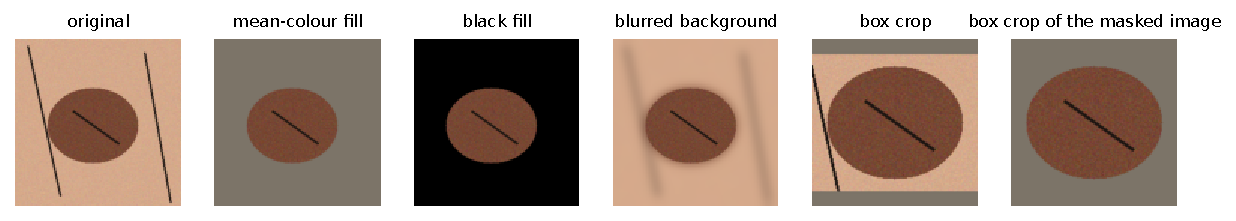
\includegraphics[width=\linewidth]{../stage7_robustness_external/figures/views_schematic.pdf}
\caption{The masking implementations of R8, illustrated on a synthetic image (a lesion with a hair-like line inside it
and two outside). No patient image is shown.}\label{s7:fig:views}\end{figure}
\paragraph{R9 --- dose-response over the real overlap} The artifact-bearing images of each cohort are binned by $r$:
$[0,0.1)$, $[0.1,0.3)$, $[0.3,0.5)$, $[0.5,0.75)$, $[0.75,1]$. Each bin is a trap with the cohort's shared artifact-free
group, built exactly like Trap~A and Trap~B. A bin with fewer than 25 images in any matched cell or fewer than 40
reversed-test positives is merged towards the middle of the $r$ range by a fixed rule. The primary endpoint is the
least-squares slope of $g_b$ on the bin's mean $r$, written as a linear combination of AUROCs so that the crossed bootstrap
gives the artifact-free images, which appear in every bin, one shared weight. H9: slope $<0$ in every cohort (Holm).
\paragraph{R10 --- ISIC 2019 $\to$ ISIC 2020} Train and validate on all \sSevenIsicTwoZeroOneNineTrainValImages{}
quality-controlled ISIC 2019 images (\sSevenIsicTwoZeroOneNineMelanomas{} melanomas) at their natural distribution; 5 seeds
of a group-safe 80/20 train/validation split. Test on every ISIC 2020 image \citep{rotemberg2021isic2020} with a lesion mask
(\sSevenIsicTwoZeroTwoZeroWithLesionMask) after removing near-duplicates of any ISIC 2019 image (perceptual hash, Hamming
distance $\le8$ --- the leakage rule of Stage~1): \sSevenTestImages{} images of \sSevenTestPatients{} patients,
\sSevenTestMelanomas{} melanomas. Lesion and hair masks are those of the Stage~5 external validation (models frozen before
any ISIC 2020 image was scored). In-lesion hair ($A$): hair on the lesion with $r\ge0.5$. Arms as in the natural test
sets of Stage~5 plus the remedies of Stage~6. Operating points OP1--OP5 use thresholds from each seed's ISIC 2019
validation predictions only. H10a: hard-pair AUROC mask $-$ ERM $<0$; H10b: at OP5 masking lowers sensitivity among
melanomas without in-lesion hair; H10c: group balancing beats masking on hard pairs.
\paragraph{R11 --- prospective theory test} The procedure of Stage~5, unchanged: for every cell (cohort $\times$ trap
or bin $\times$ arm) the two parameters $(S,A)$ are fitted to the clean and correlated AUROC, and the reversed AUROC --- and
every crossover, gain and slope built from it --- is predicted. The cells are the \sSevenTN{} R8 and R9 cells, none of which
existed when the rule was registered. Decision rule as in Stage~5: \emph{quantitatively predictive} only if every R8
crossover sign agrees, both correlations are $\ge0.7$ and the error beats ``reversed = clean''.

\subsection{Experiments}
\begin{table}[H]\centering\scriptsize
\caption{Experiments of this stage. One registration document (\texttt{docs/PREREGISTRATION\_ROUND4.md}) was committed before any feature, count or model of this stage existed. Commit times are set by the committing machine and are not independent proof of order.}\label{s7:tab:exp}
\begin{tabular}{p{3.6cm}p{3.2cm}p{2.8cm}p{5.4cm}}\toprule
Experiment & Status & First commit (local time) & Support criterion \\\midrule
R8 masking implementations (H8a, H8b) & \registered{round 4} & \texttt{d34b8b8}, 2026-09-28 11:28 & H8a: $C_v>0$ for black fill and box crop of the masked image in all four cohorts (Holm over 16) \\
R9 dose-response over the real overlap (H9) & \registered{round 4}; bin counts committed before fitting & \texttt{d34b8b8}, 2026-09-28 11:28 & slope of the mask gain on $r$ $<0$ in every cohort that passes the count gate (Holm) \\
R10 ISIC 2019 $\to$ ISIC 2020 natural test (H10a--c) & \registered{round 4} & \texttt{d34b8b8}, 2026-09-28 11:28 & hard-pair AUROC mask $-$ ERM $<0$; OP5 sensitivity loss; balancing $>$ mask on hard pairs \\
R11 prospective theory test (T1$'$--T3$'$) & \registered{round 4} & \texttt{d34b8b8}, 2026-09-28 11:28 & all crossover signs, $r\ge0.7$, MAE below ``reversed = clean'' \\
\bottomrule\end{tabular}
\end{table}


\subsection{Results}
\subsubsection{R8: the law does not depend on how masking is implemented}
Table~\ref{s7:tab:r8} and Figure~\ref{s7:fig:r8}. Every implementation gives a positive crossover in every cohort:
\sSevenNPrimOK{} of \sSevenNPrim{} tests are supported after Holm adjustment. For the full-removal views (H8a) this is
\sSevenHEightaN{} of \sSevenHEightaOf{}, so by the registered rule the law is \textbf{implementation-independent}. The
re-fitted mean-colour crossovers reproduce Stage~3 (dermoscopy \sSevenXisicmask, thyroid \sSevenXthyroidmask, capsule
\sSevenXcapsulemask, ovary \sSevenXovarymask).
\begin{table}[H]\centering\scriptsize
\caption{Location crossover $C_v$ for every masking implementation (DINOv2 ViT-B/14, crossed 95\% CIs). All 16 non-reference crossovers are positive with Holm-adjusted $p\le$ \sSevenHolmMax{} (family of 16).}\label{s7:tab:r8}
\resizebox{\linewidth}{!}{\begin{tabular}{lccccc}\toprule
Cohort & mean-colour fill (reference) & black fill & blurred background & box crop & box crop of the masked image \\\midrule
Dermoscopy hair (ISIC 2019) & $+0.147$ [$+0.111, +0.185$] & $+0.170$ [$+0.133, +0.207$] & $+0.154$ [$+0.117, +0.191$] & $+0.091$ [$+0.064, +0.117$] & $+0.154$ [$+0.121, +0.187$] \\
Thyroid calipers & $+0.239$ [$+0.196, +0.280$] & $+0.223$ [$+0.181, +0.265$] & $+0.218$ [$+0.177, +0.258$] & $+0.246$ [$+0.206, +0.285$] & $+0.250$ [$+0.210, +0.290$] \\
Capsule debris & $+0.377$ [$+0.328, +0.426$] & $+0.367$ [$+0.318, +0.416$] & $+0.278$ [$+0.221, +0.330$] & $+0.317$ [$+0.267, +0.367$] & $+0.358$ [$+0.305, +0.409$] \\
Ovary calipers & $+0.170$ [$+0.088, +0.250$] & $+0.153$ [$+0.063, +0.242$] & $+0.112$ [$+0.027, +0.195$] & $+0.145$ [$+0.083, +0.207$] & $+0.160$ [$+0.080, +0.240$] \\
\bottomrule\end{tabular}}
\end{table}

\begin{figure}[H]\centering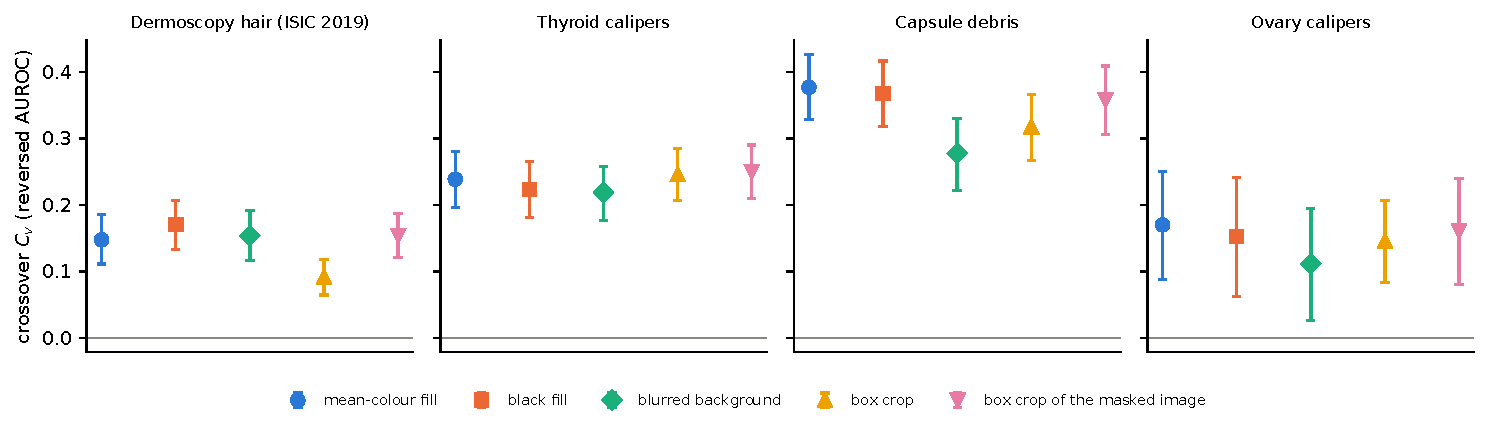
\includegraphics[width=\linewidth]{../stage7_robustness_external/figures/r8_crossover.pdf}
\caption{Crossover $C_v$ per masking implementation and cohort (crossed 95\% CIs). The reference (mean-colour fill) is
the leftmost point of each panel.}\label{s7:fig:r8}\end{figure}
\paragraph{Partial removal (H8b)} Both partial-removal views also give positive crossovers in every cohort
(\sSevenHEightbN{} of \sSevenHEightbOf), but they are weaker than mean fill only where the surviving content still
carries the artifact (Table~\ref{s7:tab:r8c}). The blurred background weakens the effect for capsule debris
(\sSevenCcapsulemaskblur) and ovarian calipers (\sSevenCovarymaskblur), not for hair (\sSevenCisicmaskblur): a 16-px blur
erases thin hair but leaves large debris recognisable. The box crop weakens it for hair (\sSevenCisiccropbox) and debris
(\sSevenCcapsulecropbox), whose out-of-ROI instances often lie next to the lesion and survive the crop, but not for
thyroid or ovarian calipers (\sSevenCthyroidcropbox, \sSevenCovarycropbox). The registered expectation ``partial removal
is weaker'' therefore holds in \sSevenHEightbConN{} of \sSevenHEightbConOf{} contrasts. One result was not expected: for hair, black fill gives a \emph{larger} crossover than mean fill
(\sSevenCisicmaskblack{} as $C_{\text{mask}}-C_v$).
\begin{table}[H]\centering\scriptsize
\caption{Secondary contrast $C_{\text{mask}}-C_v$: how much smaller the crossover of an implementation is than that of mean-colour fill (positive = weaker location effect than the reference).}\label{s7:tab:r8c}
\resizebox{\linewidth}{!}{\begin{tabular}{lcccc}\toprule
Cohort & black fill & blurred background & box crop & box crop of the masked image \\\midrule
Dermoscopy hair (ISIC 2019) & $-0.023$ [$-0.040, -0.007$] & $-0.006$ [$-0.042, +0.024$] & $+0.056$ [$+0.012, +0.099$] & $-0.007$ [$-0.033, +0.019$] \\
Thyroid calipers & $+0.016$ [$-0.004, +0.036$] & $+0.020$ [$-0.008, +0.049$] & $-0.007$ [$-0.049, +0.032$] & $-0.011$ [$-0.037, +0.014$] \\
Capsule debris & $+0.010$ [$-0.001, +0.021$] & $+0.099$ [$+0.067, +0.132$] & $+0.059$ [$+0.032, +0.087$] & $+0.019$ [$+0.001, +0.037$] \\
Ovary calipers & $+0.017$ [$-0.034, +0.079$] & $+0.058$ [$+0.004, +0.113$] & $+0.024$ [$-0.045, +0.096$] & $+0.010$ [$-0.046, +0.068$] \\
\bottomrule\end{tabular}}
\end{table}

\paragraph{What each implementation does in each trap} Figure~\ref{s7:fig:r8traps} and Table~\ref{s7:tab:r8t}. The pattern of
Stage~3 recurs for every implementation. For hair, every full-removal view harms inside the lesion (Trap~A: mean fill
\sSevenDisicmasktrapArev, black \sSevenDisicmaskblacktrapArev) and helps beside it (Trap~B: mean fill
\sSevenDisicmasktrapBrev). The views that keep some context harm less in Trap~A (blur \sSevenDisicmaskblurtrapArev, box
crop \sSevenDisiccropboxtrapArev) and gain less in Trap~B (box crop \sSevenDisiccropboxtrapBrev). For calipers and debris
every view still helps a little in Trap~A --- it removes clutter and overlays elsewhere on the screen (Stage~3) --- and
much more in Trap~B.
\begin{figure}[H]\centering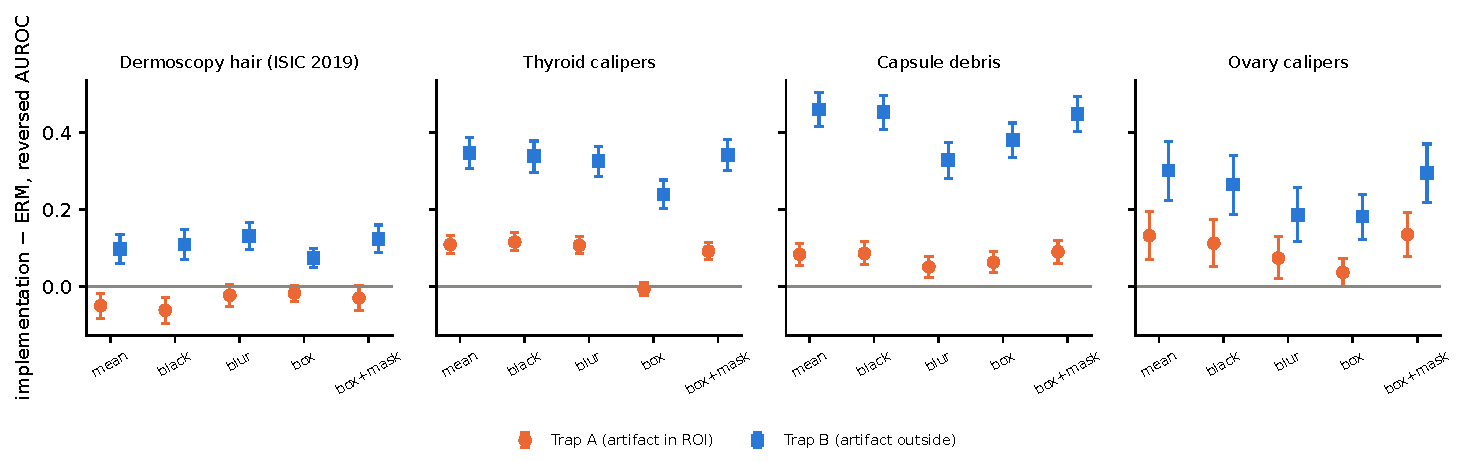
\includegraphics[width=\linewidth]{../stage7_robustness_external/figures/r8_traps.pdf}
\caption{Each implementation minus ERM on the reversed test, in Trap~A (artifact inside the ROI, orange circles) and
Trap~B (outside, blue squares); crossed 95\% CIs.}\label{s7:fig:r8traps}\end{figure}
\begin{table}[H]\centering\scriptsize
\caption{Each implementation minus ERM, per trap and test environment (AUROC, crossed 95\% CIs; descriptive).}\label{s7:tab:r8t}
\resizebox{\linewidth}{!}{\begin{tabular}{lccccc}\toprule
Cohort & Implementation & Trap~A reversed & Trap~B reversed & Trap~A clean & Trap~B clean \\\midrule
Dermoscopy hair (ISIC 2019) & mean-colour fill & $-0.049$ [$-0.083, -0.017$] & $+0.098$ [$+0.060, +0.136$] & $-0.023$ [$-0.045, -0.001$] & $-0.014$ [$-0.041, +0.014$] \\
 & black fill & $-0.061$ [$-0.097, -0.028$] & $+0.109$ [$+0.071, +0.148$] & $-0.028$ [$-0.052, -0.005$] & $-0.006$ [$-0.034, +0.022$] \\
 & blurred background & $-0.023$ [$-0.051, +0.005$] & $+0.131$ [$+0.096, +0.166$] & $-0.004$ [$-0.022, +0.014$] & $+0.020$ [$-0.006, +0.047$] \\
 & box crop & $-0.017$ [$-0.038, +0.003$] & $+0.074$ [$+0.049, +0.098$] & $-0.005$ [$-0.019, +0.009$] & $+0.010$ [$-0.007, +0.026$] \\
 & box crop of the masked image & $-0.030$ [$-0.062, +0.002$] & $+0.124$ [$+0.089, +0.160$] & $-0.010$ [$-0.030, +0.011$] & $+0.011$ [$-0.014, +0.035$] \\
Thyroid calipers & mean-colour fill & $+0.109$ [$+0.086, +0.133$] & $+0.348$ [$+0.307, +0.388$] & $+0.081$ [$+0.063, +0.100$] & $+0.166$ [$+0.118, +0.213$] \\
 & black fill & $+0.116$ [$+0.093, +0.140$] & $+0.339$ [$+0.297, +0.379$] & $+0.067$ [$+0.044, +0.089$] & $+0.171$ [$+0.125, +0.218$] \\
 & blurred background & $+0.107$ [$+0.086, +0.130$] & $+0.326$ [$+0.286, +0.365$] & $+0.065$ [$+0.044, +0.085$] & $+0.154$ [$+0.109, +0.199$] \\
 & box crop & $-0.006$ [$-0.023, +0.011$] & $+0.239$ [$+0.203, +0.277$] & $+0.015$ [$-0.003, +0.032$] & $+0.087$ [$+0.040, +0.135$] \\
 & box crop of the masked image & $+0.092$ [$+0.070, +0.115$] & $+0.342$ [$+0.303, +0.381$] & $+0.083$ [$+0.063, +0.101$] & $+0.174$ [$+0.129, +0.219$] \\
Capsule debris & mean-colour fill & $+0.084$ [$+0.055, +0.113$] & $+0.461$ [$+0.416, +0.506$] & $+0.064$ [$+0.044, +0.086$] & $+0.217$ [$+0.186, +0.251$] \\
 & black fill & $+0.086$ [$+0.056, +0.116$] & $+0.453$ [$+0.410, +0.497$] & $+0.063$ [$+0.044, +0.084$] & $+0.215$ [$+0.183, +0.248$] \\
 & blurred background & $+0.051$ [$+0.024, +0.077$] & $+0.329$ [$+0.282, +0.374$] & $+0.047$ [$+0.027, +0.068$] & $+0.156$ [$+0.129, +0.184$] \\
 & box crop & $+0.063$ [$+0.037, +0.090$] & $+0.381$ [$+0.336, +0.425$] & $+0.046$ [$+0.024, +0.068$] & $+0.174$ [$+0.145, +0.206$] \\
 & box crop of the masked image & $+0.091$ [$+0.060, +0.120$] & $+0.448$ [$+0.403, +0.494$] & $+0.056$ [$+0.033, +0.079$] & $+0.205$ [$+0.173, +0.238$] \\
Ovary calipers & mean-colour fill & $+0.132$ [$+0.071, +0.195$] & $+0.302$ [$+0.225, +0.378$] & $+0.055$ [$+0.014, +0.095$] & $+0.097$ [$+0.032, +0.159$] \\
 & black fill & $+0.113$ [$+0.053, +0.175$] & $+0.265$ [$+0.188, +0.342$] & $+0.028$ [$-0.013, +0.069$] & $+0.093$ [$+0.037, +0.149$] \\
 & blurred background & $+0.074$ [$+0.021, +0.130$] & $+0.186$ [$+0.116, +0.257$] & $+0.050$ [$+0.012, +0.086$] & $+0.065$ [$+0.014, +0.117$] \\
 & box crop & $+0.037$ [$+0.000, +0.072$] & $+0.182$ [$+0.122, +0.241$] & $+0.041$ [$+0.014, +0.068$] & $+0.078$ [$+0.038, +0.117$] \\
 & box crop of the masked image & $+0.135$ [$+0.078, +0.194$] & $+0.296$ [$+0.219, +0.371$] & $+0.050$ [$+0.007, +0.092$] & $+0.107$ [$+0.046, +0.167$] \\
\bottomrule\end{tabular}}
\end{table}


\subsubsection{R9: the location effect is graded}
Table~\ref{s7:tab:r9}, Table~\ref{s7:tab:r9b} and Figure~\ref{s7:fig:r9}. In every cohort the mask gain falls as more of the
artifact lies inside the ROI: slope \sSevenSlopeisic{} (hair), \sSevenSlopethyroid{} (thyroid), \sSevenSlopecapsule{}
(capsule) and \sSevenSlopeovary{} (ovary); \sSevenNHNine{} of \sSevenNHNineOf{} supported after Holm adjustment, with a
perfectly monotone ordering of the bins in every cohort. The two traps of Stages~3--6 are the ends of a continuous
dependence, not an artefact of the thresholds. For hair the gain passes through zero near $r=$ \sSevenZeroIsic{} and
becomes a harm when almost all of the hair lies on the lesion (\sSevenGisicbFive{} for $r\ge0.75$, against
\sSevenGisicbOne{} for $r<0.1$). For calipers and debris the gain shrinks several-fold (capsule
\sSevenGcapsulebOne{} $\to$ \sSevenGcapsulebFive; thyroid \sSevenGthyroidbOne{} $\to$ \sSevenGthyroidbFive) but stays
non-negative, for the reason given above: masking also removes on-screen clutter. The ovary cohort had too few images
with intermediate overlap and was analysed with three bins after the registered merge rule
(\sSevenBinsovary{} bins).
\begin{table}[H]\centering\scriptsize
\caption{Dose-response: least-squares slope of $g_b=$ rev(mask) $-$ rev(ERM) on the bin mean overlap $r$ (crossed 95\% CIs; the artifact-free images shared by all bins carry one bootstrap weight).}\label{s7:tab:r9}
\begin{tabular}{lcccccc}\toprule
Cohort & Bins & Slope of the mask gain on $r$ & Holm $p$ & Spearman & Zero crossing $r$ & H9 \\\midrule
Dermoscopy hair (ISIC 2019) & 5 & $-0.235$ [$-0.276, -0.194$] & $<0.001$ & -1.00 & 0.401 & \ok \\
Thyroid calipers & 5 & $-0.250$ [$-0.303, -0.197$] & $<0.001$ & -1.00 & none & \ok \\
Capsule debris & 5 & $-0.489$ [$-0.539, -0.438$] & $<0.001$ & -1.00 & none & \ok \\
Ovary calipers & 3 & $-0.205$ [$-0.300, -0.109$] & $<0.001$ & -1.00 & none & \ok \\
\bottomrule\end{tabular}
\end{table}

\begin{figure}[H]\centering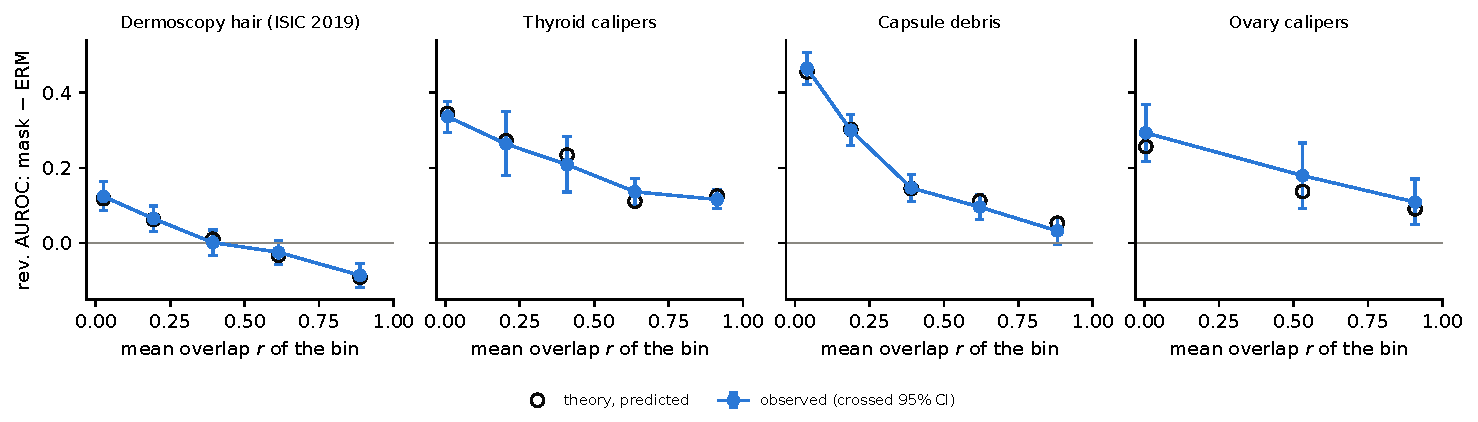
\includegraphics[width=\linewidth]{../stage7_robustness_external/figures/r9_dose.pdf}
\caption{Mask gain on the reversed test against the mean overlap $r$ of each bin (filled: observed, crossed 95\% CIs;
open: the theory's prediction from each bin's clean and correlated AUROC only).}\label{s7:fig:r9}\end{figure}
\begin{table}[H]\centering\scriptsize
\caption{Bins after the registered count gate ($\ge25$ per matched cell, $\ge40$ reversed-test positives over the folds of seed 42); merged bins are named by their parts. Cell counts are those of the matched pool.}\label{s7:tab:r9b}
\resizebox{\linewidth}{!}{\begin{tabular}{lccccccc}\toprule
Cohort & Bin & $r$ range & Mean $r$ & $A{=}1$: $Y{=}0$ / $Y{=}1$ & $A{=}0$: $Y{=}0$ / $Y{=}1$ & Rev.\ positives & Mask gain $g_b$ \\\midrule
Dermoscopy hair (ISIC 2019) & b1 & 0.00--0.10 & 0.026 & 4412 / 969 & 706 / 157 & 172 & $+0.124$ [$+0.085, +0.162$] \\
 & b2 & 0.10--0.30 & 0.194 & 3749 / 797 & 706 / 157 & 172 & $+0.065$ [$+0.029, +0.098$] \\
 & b3 & 0.30--0.50 & 0.393 & 2458 / 762 & 706 / 157 & 172 & $+0.001$ [$-0.034, +0.035$] \\
 & b4 & 0.50--0.75 & 0.614 & 1579 / 612 & 706 / 157 & 172 & $-0.025$ [$-0.057, +0.006$] \\
 & b5 & 0.75--1.00 & 0.888 & 1074 / 329 & 706 / 157 & 172 & $-0.086$ [$-0.119, -0.056$] \\
Thyroid calipers & b1 & 0.00--0.10 & 0.008 & 227 / 99 & 1052 / 749 & 829 & $+0.336$ [$+0.295, +0.377$] \\
 & b2 & 0.10--0.30 & 0.204 & 75 / 30 & 1052 / 749 & 300 & $+0.264$ [$+0.180, +0.349$] \\
 & b3 & 0.30--0.50 & 0.409 & 70 / 40 & 1052 / 749 & 400 & $+0.208$ [$+0.136, +0.283$] \\
 & b4 & 0.50--0.75 & 0.637 & 229 / 79 & 1052 / 749 & 790 & $+0.136$ [$+0.099, +0.172$] \\
 & b5 & 0.75--1.00 & 0.913 & 629 / 213 & 1052 / 749 & 829 & $+0.116$ [$+0.091, +0.141$] \\
Capsule debris & b1 & 0.00--0.10 & 0.041 & 231 / 1009 & 164 / 343 & 378 & $+0.465$ [$+0.422, +0.508$] \\
 & b2 & 0.10--0.30 & 0.188 & 391 / 769 & 164 / 343 & 378 & $+0.300$ [$+0.259, +0.343$] \\
 & b3 & 0.30--0.50 & 0.390 & 279 / 311 & 164 / 343 & 378 & $+0.147$ [$+0.111, +0.182$] \\
 & b4 & 0.50--0.75 & 0.621 & 237 / 227 & 164 / 343 & 378 & $+0.096$ [$+0.061, +0.130$] \\
 & b5 & 0.75--1.00 & 0.881 & 167 / 185 & 164 / 343 & 378 & $+0.032$ [$-0.004, +0.069$] \\
Ovary calipers & b1 & 0.00--0.10 & 0.004 & 91 / 103 & 170 / 178 & 196 & $+0.293$ [$+0.216, +0.369$] \\
 & b2b3b4 & 0.10--0.75 & 0.531 & 59 / 55 & 170 / 178 & 196 & $+0.179$ [$+0.091, +0.266$] \\
 & b5 & 0.75--1.00 & 0.909 & 298 / 244 & 170 / 178 & 196 & $+0.109$ [$+0.049, +0.170$] \\
\bottomrule\end{tabular}}
\end{table}


\subsubsection{R10: an external test at natural prevalence}
\paragraph{The data} After near-duplicate removal the test set has \sSevenTestImages{} images
(\sSevenTestMelanomas{} melanomas, \sSevenTestPatients{} patients). The removal was large: \sSevenDroppedNearDuplicates{}
images (\sSevenDropPct) were within Hamming distance 8 of an ISIC 2019 image --- \sSevenDupZerotoZero{} at distance 0,
\sSevenDupOnetoTwo{} at 1--2, \sSevenDupThreetoFive{} at 3--5 and \sSevenDupSixtoEight{} at 6--8 --- and it removed
melanomas less often (\sSevenDropMel) than benign lesions (\sSevenDropBen). Most removed images are therefore look-alikes
rather than copies (below). The association that masking can amplify is present
in both datasets: in-lesion hair on \sSevenHairisicTwoZeroOneNinemel{} of ISIC 2019 melanomas and
\sSevenHairisicTwoZeroOneNineben{} of benign lesions, and on \sSevenHairisicTwoZeroTwoZeromel{} and
\sSevenHairisicTwoZeroTwoZeroben{} in ISIC 2020.
\paragraph{AUROC} Tables~\ref{s7:tab:r10m} and \ref{s7:tab:r10b}, Figure~\ref{s7:fig:r10}. On all ISIC 2020 pairs masking
\emph{improves} the AUROC (\sSevenBmaskermall; ERM \sSevenNmermauc, mask \sSevenNmmaskauc) --- masking is the best arm by
overall AUROC. The improvement comes entirely from the shortcut-aligned pairs (\sSevenBmaskermeasy); on the
shortcut-conflicting pairs masking lowers the AUROC (\sSevenBmaskermhard; H10a \textbf{supported}, but only just: the upper
bound is \sSevenBhimaskerm). This is the Stage~5 signature --- right for the wrong reason on aligned cases, wrong on
conflicting ones --- on patients the model never saw, without any resampling. An external validation that reported only
the overall AUROC would recommend masking. Group balancing recovers the conflicting pairs (\sSevenBbalancedmaskhard{}
over mask; H10c \textbf{supported}) at a cost on aligned pairs (\sSevenBbalancedmaskeasy) and overall
(\sSevenBbalancedmaskall); combining masking with group balancing gives the highest cross-group AUROC
(\sSevenNmmaskbalancedcrossgroup, against ERM \sSevenNmermcrossgroup{} and mask \sSevenNmmaskcrossgroup).
\begin{table}[H]\centering\scriptsize
\caption{ISIC 2020 (external, natural prevalence), models trained on ISIC 2019: seed means. Hard pairs = melanomas without in-lesion hair vs benign lesions with it (they conflict with the training association).}\label{s7:tab:r10m}
\begin{tabular}{lccccc}\toprule
Arm & AUROC & Cross-group AUROC & AUROC, in-lesion hair & Hard pairs & Easy pairs \\\midrule
ERM & 0.791 & 0.772 & 0.779 & 0.772 & 0.798 \\
mask & 0.811 & 0.746 & 0.781 & 0.746 & 0.843 \\
balanced & 0.779 & 0.749 & 0.776 & 0.805 & 0.749 \\
mask + balanced & 0.792 & 0.776 & 0.777 & 0.786 & 0.783 \\
U-MtE & 0.799 & 0.752 & 0.783 & 0.752 & 0.827 \\
U-MtE balanced & 0.778 & 0.764 & 0.780 & 0.787 & 0.764 \\
U-MtE protect & 0.804 & 0.715 & 0.752 & 0.715 & 0.839 \\
U-MtE protect balanced & 0.790 & 0.753 & 0.747 & 0.753 & 0.789 \\
DFR & 0.765 & 0.730 & 0.746 & 0.782 & 0.731 \\
mask + DFR & 0.767 & 0.717 & 0.730 & 0.718 & 0.781 \\
JTT & 0.706 & 0.632 & 0.722 & 0.796 & 0.632 \\
\bottomrule\end{tabular}
\end{table}

\begin{table}[H]\centering\scriptsize
\caption{ISIC 2020: AUROC contrasts with crossed 95\% CIs (5 seeds; one Poisson weight per ISIC 2020 image).}\label{s7:tab:r10b}
\begin{tabular}{lccc}\toprule
Contrast & All pairs & Hard pairs & Easy pairs \\\midrule
mask $-$ ERM & $+0.020$ [$+0.003, +0.038$] & $-0.026$ [$-0.052, -0.000$] & $+0.045$ [$+0.005, +0.087$] \\
balanced $-$ mask & $-0.032$ [$-0.051, -0.014$] & $+0.059$ [$+0.035, +0.084$] & $-0.094$ [$-0.138, -0.051$] \\
U-MtE balanced $-$ mask & $-0.033$ [$-0.040, -0.026$] & $+0.041$ [$+0.030, +0.051$] & $-0.079$ [$-0.099, -0.059$] \\
U-MtE $-$ mask & $-0.012$ [$-0.018, -0.007$] & $+0.005$ [$-0.002, +0.013$] & $-0.016$ [$-0.029, -0.003$] \\
\bottomrule\end{tabular}
\end{table}

\begin{figure}[H]\centering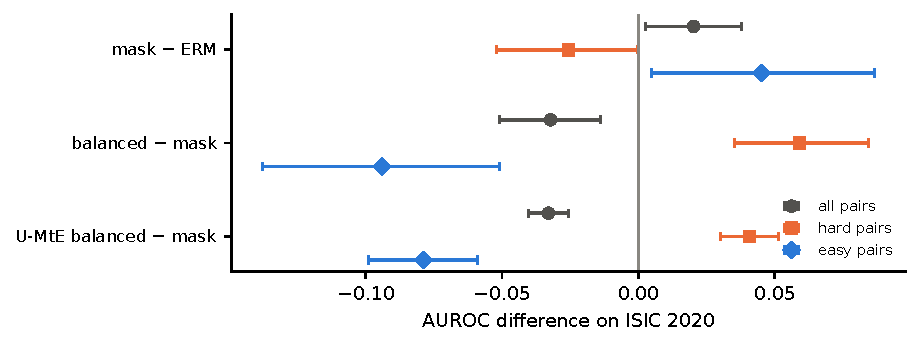
\includegraphics[width=0.75\linewidth]{../stage7_robustness_external/figures/r10_pairs.pdf}
\caption{ISIC 2020: AUROC differences on all, hard (shortcut-conflicting) and easy (shortcut-aligned) pairs; crossed
95\% CIs.}\label{s7:fig:r10}\end{figure}
\paragraph{Operating points} Table~\ref{s7:tab:r10op}. The AUROC effect does \emph{not} translate into a detectable
sensitivity loss at a fixed threshold: at OP5 (validation sensitivity $\ge0.90$) the sensitivity among melanomas without
in-lesion hair changes by \sSevenOpOPFiveconf{} (H10b \textbf{not supported}); at OP1 masking even raises sensitivity
without significance (\sSevenOpOPOnesens), and at OP2--OP4 it raises specificity (OP2 \sSevenOpOPTwospec). The clinical
consequence shown on the thyroid split of Stage~5 is therefore not reproduced here.
\begin{table}[H]\centering\scriptsize
\caption{ISIC 2020 operating points, mask $-$ ERM (crossed bootstrap with thresholds re-estimated on the weighted validation images in every replicate, 2{,}000 replicates).}\label{s7:tab:r10op}
\resizebox{\linewidth}{!}{\begin{tabular}{lccccc}\toprule
Operating point (threshold from ISIC 2019 validation) & Sensitivity ERM $\to$ mask & $\Delta$ sensitivity & $\Delta$ specificity & Sensitivity, melanomas without in-lesion hair & $\Delta$ \\\midrule
OP1 max.\ balanced accuracy & 0.434 $\to$ 0.516 & $+0.082$ [$-0.014, +0.167$] & $-0.003$ [$-0.046, +0.035$] & 0.432 $\to$ 0.519 & $+0.087$ [$-0.011, +0.168$] \\
OP2 specificity $\ge0.80$ & 0.472 $\to$ 0.477 & $+0.005$ [$-0.033, +0.052$] & $+0.029$ [$+0.017, +0.040$] & 0.470 $\to$ 0.482 & $+0.012$ [$-0.031, +0.063$] \\
OP3 specificity $\ge0.90$ & 0.309 $\to$ 0.324 & $+0.015$ [$-0.026, +0.062$] & $+0.016$ [$+0.009, +0.023$] & 0.309 $\to$ 0.332 & $+0.023$ [$-0.024, +0.072$] \\
OP4 sensitivity $\ge0.80$ & 0.523 $\to$ 0.545 & $+0.022$ [$-0.033, +0.077$] & $+0.021$ [$+0.002, +0.039$] & 0.524 $\to$ 0.547 & $+0.022$ [$-0.031, +0.079$] \\
OP5 sensitivity $\ge0.90$ & 0.702 $\to$ 0.699 & $-0.003$ [$-0.055, +0.052$] & $+0.028$ [$-0.011, +0.060$] & 0.700 $\to$ 0.693 & $-0.007$ [$-0.060, +0.047$] \\
\bottomrule\end{tabular}}
\end{table}


\subsubsection{R11: the theory predicts results it had not seen}
Table~\ref{s7:tab:r11} and Figure~\ref{s7:fig:r11}. Fitted only to each cell's clean and correlated AUROC, the theory's
predictions of the \sSevenTN{} held-out reversed AUROCs have a mean absolute error of \sSevenTMae{} (Pearson $r=$
\sSevenTR; \sSevenTWithin{} within 0.05), against \sSevenTMaeSym{} for the symmetric-reversal heuristic and
\sSevenTMaeClean{} for ``reversed = clean''. It gets the sign of all \sSevenTTwoN{} R8 crossovers right (\sSevenTTwoSign{} of
\sSevenTTwoN; $r=$ \sSevenTTwoR, MAE \sSevenTTwoMae), the sign of \sSevenTThreeSign{} of \sSevenTThreeN{} dose-response slopes
(MAE \sSevenTThreeMae) and of \sSevenTBinSign{} of \sSevenTBinN{} bin gains. By the registered rule the verdict is
\textbf{\sSevenTVerdict}. The difference from Stage~5's verdict (a qualitative account) is one of scope, not of rule:
Stage~5's cell set included chest radiographs, where one near-zero crossover had the wrong sign; the cells here are frozen
DINOv2 encoders with linear heads on four cohorts --- the setting the theory assumes.
\begin{table}[H]\centering\scriptsize
\caption{Prospective theory test: fitted to each cell's clean and correlated AUROC only; the reversed AUROC and every quantity derived from it are held out. None of these cells existed when the rule was registered.}\label{s7:tab:r11}
\begin{tabular}{lcccc}\toprule
Endpoint & Cells & Theory & ``reversed = clean'' & Symmetric reversal \\\midrule
T1$'$ reversed AUROC, all new cells & 84 & MAE 0.011, $r=$ 0.996 & MAE 0.177 & MAE 0.036 \\
T2$'$ R8 crossovers & 16 & signs 16/16, $r=$ 0.992, MAE 0.011 &  &  \\
T3$'$ R9 slopes & 4 & signs 4/4, MAE 0.018 &  &  \\
T3$'$ R9 bin gains & 18 & signs 18/18, MAE 0.014 &  &  \\
\bottomrule\end{tabular}
\end{table}

\begin{figure}[H]\centering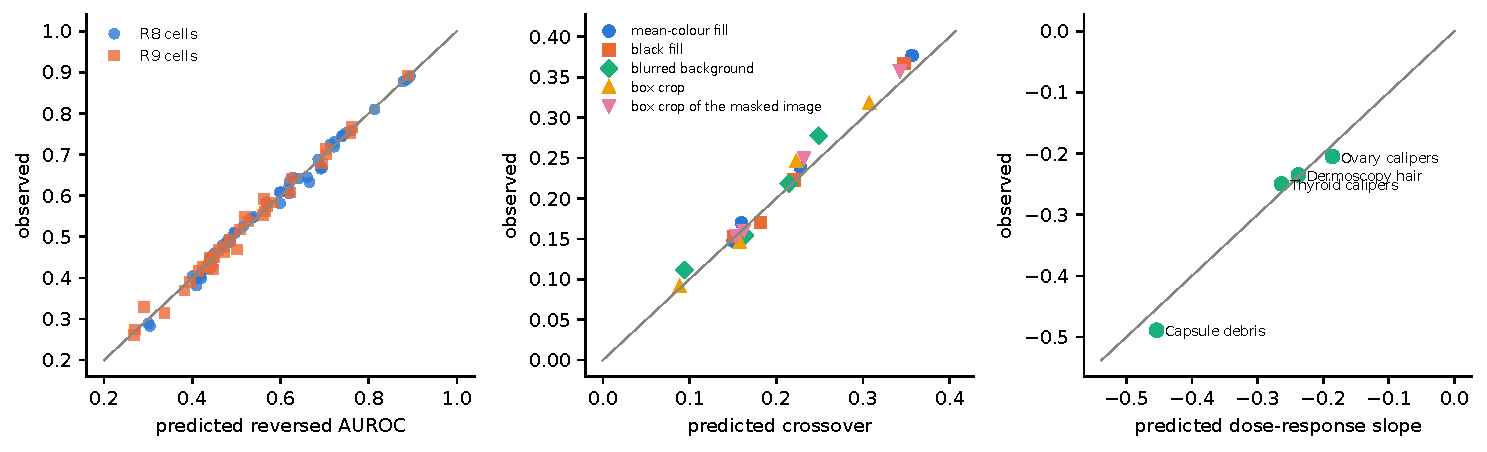
\includegraphics[width=\linewidth]{../stage7_robustness_external/figures/r11_theory.pdf}
\caption{Prospective test of the theory. Left: predicted versus observed reversed AUROC for every R8 and R9 cell. Middle:
R8 crossovers. Right: R9 dose-response slopes. Grey lines are the identity.}\label{s7:fig:r11}\end{figure}

\subsection{What failed or changed}
\begin{itemize}[leftmargin=*]\itemsep1pt
\item \textbf{H8b} holds in \sSevenHEightbConN{} of \sSevenHEightbConOf{} contrasts: partial removal is weaker than mean
fill for debris and ovarian calipers (blur) and for hair and debris (box crop), not otherwise; black fill gives a larger
hair crossover than mean fill.
\item \textbf{H10a} is supported by a margin that disappears at the third decimal; \textbf{H10b} is not supported: on
ISIC 2020 masking does not measurably lower sensitivity at a fixed operating point.
\item \textbf{Near-duplicate removal} discarded \sSevenDropPct{} of ISIC 2020. The rule was registered and uses no labels,
but \sSevenDupSixtoEight{} of the \sSevenDroppedNearDuplicates{} removed images are at distance 6--8, where a perceptual
hash also matches merely similar dermoscopy images, and melanomas were removed less often than benign lesions; the test
set is smaller than necessary, and a sensitivity analysis with a stricter distance was not run.
\item \textbf{The ovary} dose-response has only three bins.
\item \textbf{Scope}: R8--R10 use one encoder (DINOv2 ViT-B/14); R10 is dermoscopy only; the prospective theory test
covers frozen-encoder linear heads only.
\item No deviation from the registration. During the run only the execution was changed (parallel head fitting and
bootstraps, one BLAS thread per process, feature extraction in a separate process, batch size 128 for the new views);
data, seeds, models, estimands and bootstrap replicates are those registered, and the reproducibility gate was passed
exactly.
\end{itemize}

\subsection{Anticipated questions}
\paragraph{Why test several masking implementations if the theory already says what masking does?} Because the theory
treats masking abstractly (it lowers the disease signal and removes the out-of-ROI artifact signal). Real implementations
differ in what they leave behind --- a black border, blurred context, nearby pixels --- and a reviewer can reasonably
suspect that one of them escapes the law. None does.
\paragraph{Why does blur work as well as mean fill for hair but not for debris?} A 16-px Gaussian blur removes structures
a few pixels wide --- hair --- almost completely, so for hair it is effectively full removal. Capsule debris and bubbles
are large, low-frequency blobs that remain recognisable after blurring, so part of the out-of-ROI shortcut survives
(\sSevenCcapsulemaskblur{} weaker crossover).
\paragraph{Why is black fill stronger than mean fill for hair?} Not established. Black fill removes slightly more disease
context than mean fill inside Trap~A (clean AUROC \sSevenDisicmaskblacktrapAclean{} against \sSevenDisicmasktrapAclean{}) and
gains slightly more in Trap~B, which widens the crossover; why a black background does this for DINOv2 was not examined.
\paragraph{Why do the thyroid, capsule and ovary gains stay positive at $r\approx0.9$?} Masking removes more than the
artifact: on-screen annotations, scanner overlays and clutter outside the ROI also carry label information in the
training environment (Stage~3). The location law is about the part of the gain that the artifact's position controls, and
that part falls monotonically; for hair, where masking also removes disease context (Stage~2), the net gain becomes a harm.
\paragraph{Why is masking the best arm on ISIC 2020 by overall AUROC if it amplifies a shortcut?} Because the shortcut
agrees with the label in ISIC 2020 too: in-lesion hair is more common on melanomas. A model that relies more on in-lesion
hair gains on the many aligned pairs and loses on the fewer conflicting ones, and the aligned pairs dominate the overall
AUROC. This is exactly why the location law matters for external validation: the harm is invisible in the headline metric.
\paragraph{Why is the AUROC harm not visible at the operating points?} The hard-pair AUROC compares melanomas without hair
with benign lesions \emph{with} hair; a fixed threshold instead compares each melanoma with a threshold learned on ISIC
2019. Masking moved that threshold (specificity rises at OP2--OP4), and with \sSevenTestMelanomas{} melanomas the
sensitivity intervals are wide. On the thyroid split of Stage~5 the loss was large enough to show at every operating point;
on ISIC 2020 it is not.
\paragraph{Why were so many ISIC 2020 images removed, and does it matter?} The registered rule removes any ISIC 2020 image
within Hamming distance 8 of any ISIC 2019 image, the same threshold used to group near-duplicates for leakage-safe splits
(Stage~1). Dermoscopy images share a global layout (a central dark lesion on skin), so at distances 6--8 the hash also
matches different images. Only \sSevenDupZerotoZero{} removed images were exact
copies; \sSevenDupSixtoEight{} were at distance 6--8. The rule errs on the side of removing leakage and uses no labels, but
it removed melanomas less often than benign lesions (\sSevenDropMel{} against \sSevenDropBen), so it slightly raised the
melanoma share of the test set. Whether the hard-pair effect depends on it can be checked with a stricter distance.
\paragraph{Does the ``quantitatively predictive'' verdict replace Stage~5's ``qualitative account''?} No. Each verdict
belongs to its registered cell set. The defensible statement is: across all cohorts (Stage~5) the theory is a qualitative
account; for frozen-encoder linear heads on the four real-artifact cohorts it predicted \sSevenTN{} new cells
prospectively within \sSevenTMae{} AUROC and met the registered criterion.

\subsection{Conclusion}
\textbf{Supported.} The location crossover is independent of the masking implementation (\sSevenNPrimOK{} of \sSevenNPrim{} tests; H8a \sSevenHEightaN{} of \sSevenHEightaOf); it is
graded in the real overlap in all four cohorts (H9); on an external, patient-level test set at natural prevalence
masking lowers the AUROC on shortcut-conflicting pairs while raising it overall (H10a, borderline), and group balancing
recovers those pairs (H10c); the theory met its registered criterion for quantitative prediction on \sSevenTN{} prospective
cells. \textbf{Qualified.} Partial-removal views are weaker than mean fill in only \sSevenHEightbConN{} of \sSevenHEightbConOf{} contrasts (H8b), the
external AUROC harm is small, and near-duplicate removal was aggressive. \textbf{Not supported.} A sensitivity loss at a
fixed operating point on ISIC 2020 (H10b).

\subsection{Questions for the supervisor}
\begin{enumerate}\itemsep1pt
\item Should the masking-implementation result (R8) and the dose-response (R9) enter the main text, as the direct answers
to ``is mean fill a strawman?'' and ``are the traps hand-picked?''?
\item Is the ISIC 2020 result --- overall improvement, conflicting-pair harm, no operating-point effect --- best presented
as an argument for subgroup reporting in external validation rather than as a clinical harm?
\item May the paper now say that the theory \emph{predicts} for frozen-encoder linear probes, keeping ``qualitative
account'' for the full cell set?
\item Should the near-duplicate sensitivity analysis (a stricter hash distance) be run before submission?
\end{enumerate}

